%-*-latex-*-
%-*-latex-*-
\newcommand\COURSE{ciss245}
\newcommand\ASSESSMENT{q2605}
\newcommand\ASSESSMENTTYPE{Quiz}
\newcommand\POINTS{\textwhite{xxx/xxx}}

\input{myquizpreamble}
\input{yliow}
\input{\COURSE}
%-*-latex-*-

%-*-latex-*-

%-*-latex-*-
\renewcommand\TITLE{\ASSESSMENTTYPE \ \ASSESSMENT}

\renewcommand\EMAIL{}
\renewcommand\AUTHOR{YOUR EMAIL}

\textwidth=6in
\begin{document}
\topmatterthree

%-*-latex-*-
\textsc{Instructions}
\begin{enumerate}
\li This is a closed-book, no-discussion, no-calculator, no-browsing-on-the-web
    no-compiler/no-MIPS-simulator test.
\li Cheating is a serious academic offense. If caught you will 
    receive an immediate score of -100\%.
\li If a question asks for a program output and the program or
    code fragment contains
    an error, write \verb!ERROR! as output.
    When writing output, whitespace is significant.
\li If a question asks for the computation of a value and the program or
    code fragment contains
    an error, write \verb!ERROR! as value.
\li When you're asked to write a C++ statement, don't forget that it must
    end with a semicolon.
\li Bubblesort refers to the bubblesort algorithm in our notes
    where values are sorted in ascending order.
\end{enumerate}

\vspace{1cm}


\begin{center}
  \textsc{Honor Statement}
\end{center}
I, \answerbox{Brysen Landis},
attest to the fact that the submitted work is my own and
is not the result of plagiarism.
Furthermore, I have not aided another student in the act of
plagiarism.

% ------------------------------------------------------------------------------
\begin{python}
from scoretable import *
\end{python}
        
%-------------------------------------------------------------------------------
\newpage
\nextq
Complete the following program. You can only add to the given code.
You cannot delete or change what is given below.

\textsc{Answer:}
\begin{answercode}
#include <iostream>

void swap(int * p, int * q)
{
    int t;
    t = *q;
    *q = *p;
    *p = t;
}


int main()
{
    int x = 0;
    int y = 1;

    swap(x, y);
    
    std::cout << x << ' ' << y << '\n'; // expected output: 1 0
    
    return 0;
}
\end{answercode}

% ------------------------------------------------------------------------------
\newpage
\nextq
Complete the following program.
You can only add to the given code. 
You cannot delete or change what is given below.

The function \verb!reverse(x, x_len)! reverses the values in the integer
array \verb!x!
from index \verb!0! up to index \verb!x_len - 1!.
For instance suppose the user enters \verb!2 3 5 7 -9999!, then
the values \verb!2, 3, 5, 7! are placed in \verb!x!
and \verb!x_len! is set to 4.
After calling \verb!reverse(x, x_len)!,
the first four value in \verb!x! becomes \verb!7, 5, 3, 2!.

\textsc{Answer:}
\begin{answercode}
#include <iostream>

void reverse(int x[], int x_len)
{
       int l = 0;
       int r = x_len - 1;
       
       while (l < r)
       {
         x[l] = x[r];
         ++l;
         --r;
       }

       return;
}


int main()
{
    int x[1024];
    int x_len;

    x_len = 0;
    for (int i = 0; i < 1024; ++i)
    {
        int t;
        std::cin >> t;
        if (t == -9999)
        {
            break;
        }
        x[x_len] = t;
        ++x_len;
    }

    reverse(x, x_len);
    // x from index 0 to x_len - 1 is now reverse.
    
    return 0;
}
\end{answercode}

% ------------------------------------------------------------------------------
\newpage
\nextq
What is the output of this program?
\begin{Verbatim}[frame=single]
int x = 10;
int y = 20;
int * p = &x;
int * q = &y;
*p = *p * *q;
*q = 42;
std::cout << x << ' ' << y << '\n';
std::cout << *p << ' ' << *q << '\n';
\end{Verbatim}

\textsc{Answer:}
\begin{answercode}
200 42
200 42
\end{answercode}

%-------------------------------------------------------------------------------
\newpage
\nextq
Rewrite the following code fragment by doing the following: Do a simple addition
program using the following skeleton.
You MUST follow the given instructions.

\textsc{Answer:}
\begin{answercode}
int x = 0, y = 0;
int * p = &x;
int * q = &y;

std::cin >> *p;
std::cin >> *q;

std::cout << x + y << '\n';
\end{answercode}

%-------------------------------------------------------------------------------
\newpage
\nextq
What is the output of this code fragment?
\begin{Verbatim}[frame=single]
int i = 1;
int j = 2;
int k = 3;
int * p = &i;
int * q = &j;
int * r = &k;
p = q;
q = r;
std::cout << *p << ' ' << *q << ' ' << *r << '\n'; 
\end{Verbatim}

\textsc{Answer:}
\begin{answercode}
2 3 3
\end{answercode}

%-------------------------------------------------------------------------------
\newpage
\nextq
You were brainstorming with your team in one of the company's meeting rooms.
Your boss popped in to say hi on his way to get coffee and
he noticed the following diagram on the whiteboard.
Someone was tracing a piece of code on the whiteboard:
\begin{center}
  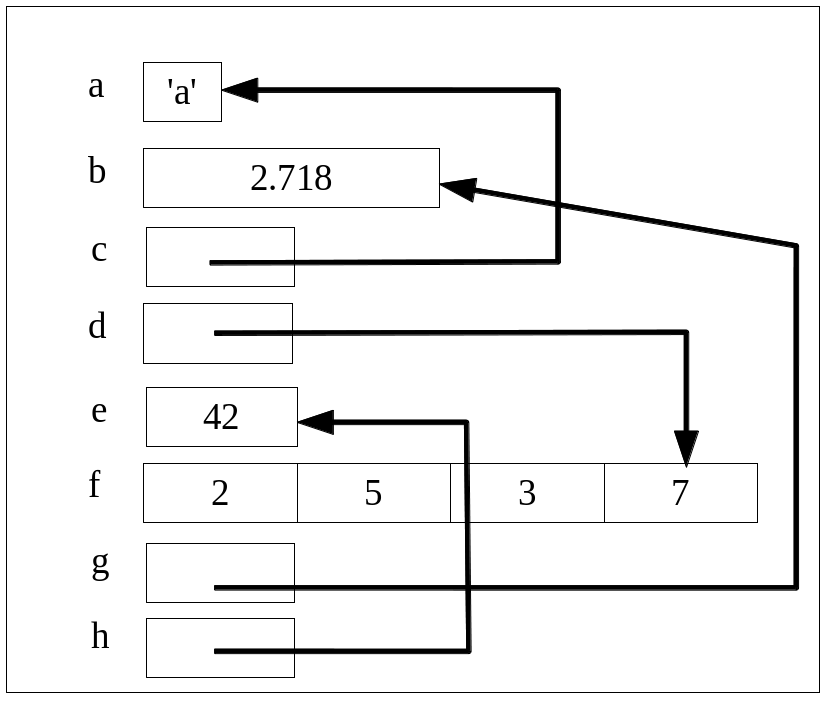
\includegraphics[width=3in]{pic1.PNG}
\end{center}
On his way back, your boss glanced at the whiteboard and saw this:
\begin{center}
  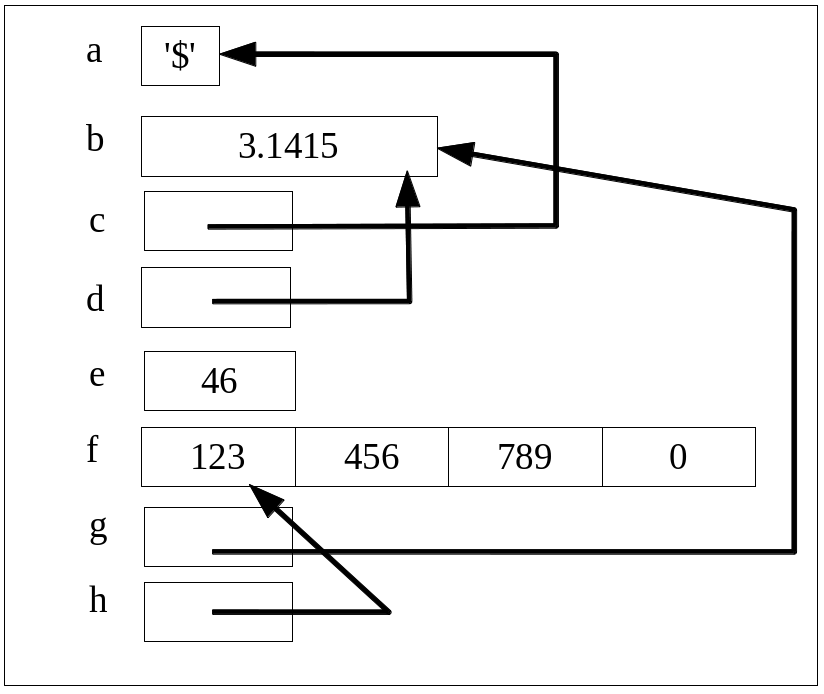
\includegraphics[width=3in]{pic2.PNG}
\end{center}
You noticed he was shaking his head as he walked away. Why?

\textsc{Answer:}
\begin{answercode}
The values within the variables a, b, e, f are changing.
(I'm honestly very confused with this one.)
\end{answercode}

%-------------------------------------------------------------------------------
\newpage
\nextq
The following program does compile and does run. But it has a memory leak.
Fix it so that there is no memory leak.

\textsc{Answer:}
\begin{answercode}
#include <iostream>

int sum(int n)
{
    int s = 0;
    int * i = new int;
    for (*i = 0; *i <= n; ++(*i))
    {
        s += *i;
    }
    delete i;
    return s;
}

int main()
{
    std::cout << sum(10) << '\n';
    return 0;
}
\end{answercode}

%-------------------------------------------------------------------------------
\newpage
\nextq
The following program get two integer values from the user 
and then prints the sum.
Do NOT use integer or double variables -- you can only use pointers.
In fact I have already declared all the variables you need,
i.e., two pointer variables.
You must allocate and deallocate memory correctly.

\textsc{Answer:}
\begin{answercode}
#include <iostream>

int main()
{
    int * p;
    int * q;

    *p = new int;
    *q = new int;

    std::cin >> *p;
    std::cin >> *q;

    std::cout << *(p) + *(q) << '\n'; 

    delete q;
    delete p;


    return 0;
}
\end{answercode}

%-------------------------------------------------------------------------------
\newpage
\nextq
Complete this code segment.

\textsc{Answer:}
\begin{answercode}
int x[] = {1, 5, 3, 7, 9, 4, 2, 6, 8, 0};
int max;

int * start = &x[0];
int * end = &x[10];
int * p;
int * pmax = &max;
// Complete the following to compute the maximum value in the array x
// from *start to *(end - 1) and store it in variable max.
// Your code must work for different array values in x.
// You also cannot use the name x or max.
// You must use a loop (of course).
// You can only use integer pointer variables start, end, p, pmax

for (*start; *start < *(end - 1); ++start)
{
  if (*start < *(start + 1))
  {
    *pmax = *(start + 1)
  }
}

// At this point the maximum value of *start,...,*(end - 1) is stored in
// variable max.
std::cout << max << '\n';
\end{answercode}

%-------------------------------------------------------------------------------
\newpage
\nextq
The following have a function that attempts to perform memory allocation
and memory deallocation, but
they are done incorrectly:
\vspace{-3mm}
\begin{Verbatim}[frame=single,fontsize=\small]
void mynew(int * p)
{
    p = new int;
}

void mydelete(int * p)
{
    delete p;
    p = NULL;
}

int main()
{
    int * p;
    mynew(p);
    *p = 42;
    mydelete(p);
    if (p != NULL) std::cout << "ERROR\n";
    
    return 0;
}
\end{Verbatim}
\vspace{-5mm}Fix the above problem below.

\textsc{Answer:}\vspace{-3mm}
\begin{answercode}
void mynew(int *p)
{
  *p = new int;
}

void mydelete(int *p)
{
  *p = NULL;
}

int main()
{
    int * p;
    mynew(p);
    *p = 42;
    mydelete(p);
    return 0;
}
\end{answercode}

%-------------------------------------------------------------------------------
\newpage
\nextq
Complete the following by writing a struct and making any corrections.
\\
\textsc{Answer:}\vspace{-2mm}
\begin{answercode}
#include <iostream>

// define the struct here
struct Student
{
  int student_id;
  int dob_year;
  int dob_month;
  int dob_day;
  int height;
  int weight;
};


void input(Student * x)
{
    std::cin >> x->student_id; // get an integer value from user for x's 
                              // student id
    std::cin >> x->dob_year;   // get an integer value from user for x's year 
                              // of date of birth
    std::cin >> x->dob_month;  // get an integer value from user for x's month 
                              // of date of birth
    std::cin >> x->dob_day;    // get an integer value from user for x's day 
                              // of date of birth
    std::cin >> x->height;     // get a double value from user for x's height
    std::cin >> x->weight;     // get a double value frin user for x's weight
}


void print(Student & x)
{
  std::cout << x->student_id << ','
            << x->dob_year << ','
            << x->dob_month << ','
            << x->dob_day << ','
            << x->height << ','
            << x->weight << '\n';
}


int main()
{
    Student john;
    input(john);
    println(john); // print all values of john separated by ',' and print '\n'
    return 0;
}
\end{answercode}

%-------------------------------------------------------------------------------
\newpage
\nextq
You are writing a tic-tac-toe game. The following code is in your
\verb!main()!:
\vspace{-3mm}
\begin{Verbatim}[frame=single,fontsize=\small]
#include <iostream>
#include "TTT.h"

int main()
{
    TTT board;

    while (1)
    {
        print(board);
        int row, col;
        get_input(board, row, col);
        make_move(board, row, col);
        if (game_ended(board)) 
        {
            break;
        }
    }
    print_result(board);

    return 0;
}
\end{Verbatim}
\vspace{-4mm}
Complete the header file (with the struct definition and the function
prototypes -- no function body definitions).
The struct and function prototypes must be minimal
(i.e., no useless member variables, no unnecessary parameters,
reference parameters must be constant whenever possible).

\textsc{Answer:}\vspace{-2mm}
\begin{answercode}
#ifndef TTT_H
#define TTT_H

struct TTT
{
  int board[9];
  int row;
  int col;
};

void print(const int &board[]);
int get_input(const int &board[], int, int);
int make_move(int &board[], int, int);
const int game_ended(const int &board);
void print_result(print());

#endif
\end{answercode}

%-------------------------------------------------------------------------------
\newpage
\nextq
What is the output? Or is there an error?
\begin{Verbatim}[frame=single,fontsize=\small]
#include <iostream>

int h(int * p)
{
    return *p;
}

int * g(int * p)
{
    return p;
}

int * f(int * p)
{
    return (p != NULL ? g(p) : NULL);
}

int main()
{
    int i = 5;
    std::cout << *f(&i) + h(&i) << std::endl;
    return 0;
}
\end{Verbatim}

\textsc{Answer:}\vspace{-2mm}
\begin{answercode}
ERROR
\end{answercode}

%-------------------------------------------------------------------------------
\newpage
\nextq
Complete the following program. Make sure there is no memory leak.

\textsc{Answer:}\vspace{-3mm}
\begin{answercode}
#include <iostream>

int f(int n)
{
    int * p;

    // Allocate an integer array of size n to p. (Of course the array
    // is in the heap.)
    
    p = new int[n];

    // Fill the array that p points to with values 1, 2, 3, ..., n.

    for (p; p < n; ++i)
    {
      std::cin >> x[*p];
    }

    // Go over the values in the array that p points to and 
    // (1) if a value is odd, replace that value by the square root of the
    //     value, or
    // (2) if a value x is even, replace that value x by x + 1. 
    // This is one pass.
    // Repeat this until every value in the array is <= 42.
    // Return the number of passes you have to run over the array

    int ret; // number of passes

    return ret;
}

int main()
{
    int n;
    std::cin >> n;
    std::cout << f(n) << '\n';
    return 0;
}
\end{answercode}

%-------------------------------------------------------------------------------
\newpage
\nextq
Complete the following function that performs the binary search.
You need NOT use recursion.
    
\textsc{Answer:}\vspace{-2mm}
\begin{answercode}
// Performs binary search on *start, *(start+1), ..., *(end - 1) for the
// value of target and return the pointer where target is found.
// If target is not found, NULL is returned.
int * binarysearch(int * start, int * end, int target)
{
  int mid = (end - start) / 2;
  while (start < end)
  {
    if (mid == target)
    {
      return mid;
    }
    else if (mid > target)
    {
      mid = mid - 1;
    }
    else
    {
      return NULL:
    }
  }

}
\end{answercode}

%-------------------------------------------------------------------------------
\newpage
\nextq
Complete the program below. Here are two test cases.
\\
\textsc{Test 1}
\begin{console}[commandchars=\\\{\}]
\userinput{1 2 3}
\userinput{4 5 6}
4 5 6
1 2 3
\end{console}
\textsc{Test 2}
\begin{console}[commandchars=\\\{\}]
\userinput{10 9 8}
\userinput{5 6 7}
5 6 7
10 9 8
\end{console}

\textsc{Answer:}\vspace{-2mm}
\begin{answercode}
#include <iostream>

void swap(int ** p, int ** q))
{
    int t = **q;
    **q = **p;
    **p = t;
    return;
}

int main()
{
    int * p = new int[3];
    int * q = new int[3];
    for (int i = 0; i < 3; ++i)
    {
        std::cin >> p[i];
    }
    for (int i = 0; i < 3; ++i)
    {
        std::cin >> q[i];
    }

    swap(&p, &q);
    for (int i = 0; i < 3; ++i)
    {
        std::cout << p[i] << ' ';
    }
    std::cout << '\n';
    for (int i = 0; i < 3; ++i)
    {
        std::cin << q[i] << ' ';
    }
    std::cout << '\n';
    delete [] p;
    delete [] q;
    return 0;
}
\end{answercode}

%------------------------------------------------------------------------------
\newpage
\input{instructions}
\end{document}
